%presentation.tex
%Andy Sayler
%Constantin Berzan
%-----------------------------------------------------------------------------%
\documentclass[xcolor=dvipsnames]{beamer}
%\useoutertheme{default}
%\usetheme{Boadilla}
\setbeamercovered{transparent=25}
\setbeamertemplate{blocks}[rounded][shadow=false] 
\setbeamertemplate{navigation symbols}{}
\usepackage{graphics}

\title[SLAM]{More SLAM}
%\subtitle[]{}
\author[ C. Berzan \& A. Sayler]{ Constantin Berzan \& Andy Sayler}
\institute[Tufts University]{
  Tufts University\\
  COMP150 - BBR\\
  \texttt{constantin.berzan@tufts.edu}\\
  \texttt{andrew.sayler@tufts.edu}
}
\date[Dec. 14, 2010]{Tuesday, December 14\textsuperscript{th}, 2010}

\begin{document}
  
  %----Title Slide------------------------------------------------------------%
  \begin{frame}[plain]
    \titlepage
  \end{frame}
  
  \section*{Outline}  
  %----Outline Slide----------------------------------------------------------%
  \begin{frame}{Outline}
    \pause
    \tableofcontents[pausesections]
  \end{frame}
  
  \section{Overview}
  %----SLAM Overview - Andy--------------------------------------------------%
  \begin{frame}{SLAM Overview}
    
  \end{frame}
  
  \section{Landmarks}
  %----Landmarks - Constantin--------------------------------------------------%
  \begin{frame}{Landmarks}
    
  \end{frame}

  {
  \usebackgroundtemplate{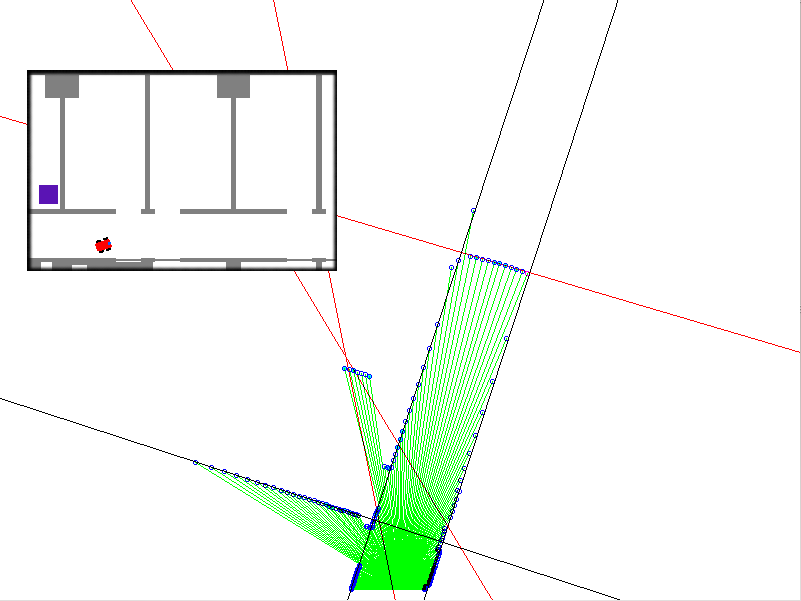
\includegraphics[width=\paperwidth]{ransac-mix.png}}
  \begin{frame}{Line extraction example}
  \end{frame}
  }

  \section{EKF}
  %----EKF - Andy--------------------------------------------------%
  \begin{frame}{EKF}
    
  \end{frame}
  
  \section{Demo}
  %----Demo - Both--------------------------------------------------%
  \begin{frame}{Demo}
    
  \end{frame}
  

\end{document}
